\section{Evaluation}
\label{sec:evaluate}

This section evaluates the costs of the various layers of abstraction in our platform.
We evaluate the cost of these layers using a set of micro-benchmarks, written
in both C++ and Static TypeScript, with three microcontrollers (Table~\ref{table:devices}): nRF51 (micro:bit),
SAMD21 (CPX device), and Atmega (Uno). The C++ benchmarks isolate the performance
of \CO and provide a baseline, while the Static TypeScript benchmarks show the overhead
added by \MC.

%add some words here about upcoming results... after order is finalised

\begin{table}[]
\centering

\begin{tabular}{c|c|c|}
\cline{2-3}
\multicolumn{1}{l|}{}             & micro:bit       & CircuitPlayground \\ \cline{2-3}
\multicolumn{1}{l|}{}             & Time Taken (ms) & Time Taken (ms)   \\ \hline
\multicolumn{1}{|c|}{\CO}       & 102             & 30.94             \\ \hline
\multicolumn{1}{|c|}{\MC}    & 216.8           & 747.2             \\ \hline
\multicolumn{1}{|c|}{micropython} & 10000           & 5679              \\ \hline
\multicolumn{1}{|c|}{Espruino}    & 115600          & -                 \\ \hline
\end{tabular}
\caption{\label{table:vm-comparison} A comparison between fully virtualised solutions, \MC, and native C++.}
\end{table}

\subsection{Software \& Devices}

The C++ of our platform breaks into two essential layers:
\begin{itemize}
\item \emph{\CON-core}: the \CO device runtime, against which we write C++ programs;
\item \emph{\MCN-common-packages}: the C++ and Static TypeScript wrapping \CON-core
to make it known to \MC, against which we write Static TypeScript programs;
\end{itemize}
%some expansion required
\MC and \CO currently runs on three different devices (Table~\ref{table:devices}), each with varying capabilities. The simplest device is the Uno, consisting of an 8-bit processor running at 48 MHz, it only has 2kB of RAM (a thousandth of the amount a smartphone has in 2017) and 32kB of flash. The Uno has no onboard components other than the microcontroller which supports: GPIO, Serial, and I2C. The micro:bit is a 32-bit cortex M0 clocking at 16MHz, with 16kB RAM and 256kB of flash. It has a number of onboard components including: a 5x5 LED matrix display, a compass, accelerometer, buttons, GPIO, I2C, Serial, and Bluetooth Low Energy. The CircuitPlayground is a 32-bit cortex M0 plus, which offers greater energy efficiency and performance, it clocks at 48 MHz and has 32kB of RAM and 256kB of flash. On board the CircuitPlayground are: RGB pixels, an infrared transmitter and receiver, a touch sensor, buttons, accelerometer, speaker, microphone, GPIO, I2C, and Serial. The solution for the micro:bit takes the untagged strategy, whilst the solution for the CircuitPlayground takes the tagged strategy (See Section~\ref{sec:untagged-tagged}).

\subsection{Methodology}

To analyse the performance of our solution, we have written a suite of programs to evaluate different aspects of the platform. Although the content of the programs differs, the approach remains the same:

\begin{enumerate}
    \item \textit{Performance Analysis}: Tests that capture time taken to perform an operation will toggle a GPIO before executing the operation, execute the operation, and toggle the GPIO at the end of the operation. Using an oscilloscope, we can then determine the time taken to perform that operation.

    \item \textit{Memory Analysis}: Tests that capture the RAM footprint of a certain operation will print a map of memory before executing the operation, execute the operation, and print a map of memory at the end of the operation. A serial terminal is used to capture the output of these tests.
\end{enumerate}

It is important to note that memory and performance analysis are tested separately, as outputting data over a serial port directly affects timing.

\subsection{Contextualising \MC and \CO}

To contextualise the \MC approach within the space, we perform a comparitive evaluation against fully virtualised solutions using native C++ as our baseline.

We devised a program to give the cost of each solutions' abstraction with respect to time. The program counted from 0 to 100000 in a tight for loop, toggling a GPIO at the beginning and end of the for loop; we measured the duration using an oscilloscope. The program was rewritten in each solutions' respective language and are functionally equivalent, the results are shown in Table~\ref{table:vm-comparison}.

For the micro:bit, micropython and Espruino are an order of magnitude slower than a native \CO program, whilst \MC is only 114 milliseconds slower. However, \MC for the CircuitPlayground takes the tagged approach to memory management, and runs almost four times slower than a micro:bit whilst executing instructions three times as fast. For both devices, \MC outperforms virtualised solutions.

\subsection{Scheduler Performance}

\subsubsection{Context Switch}

\begin{figure}[ht]
    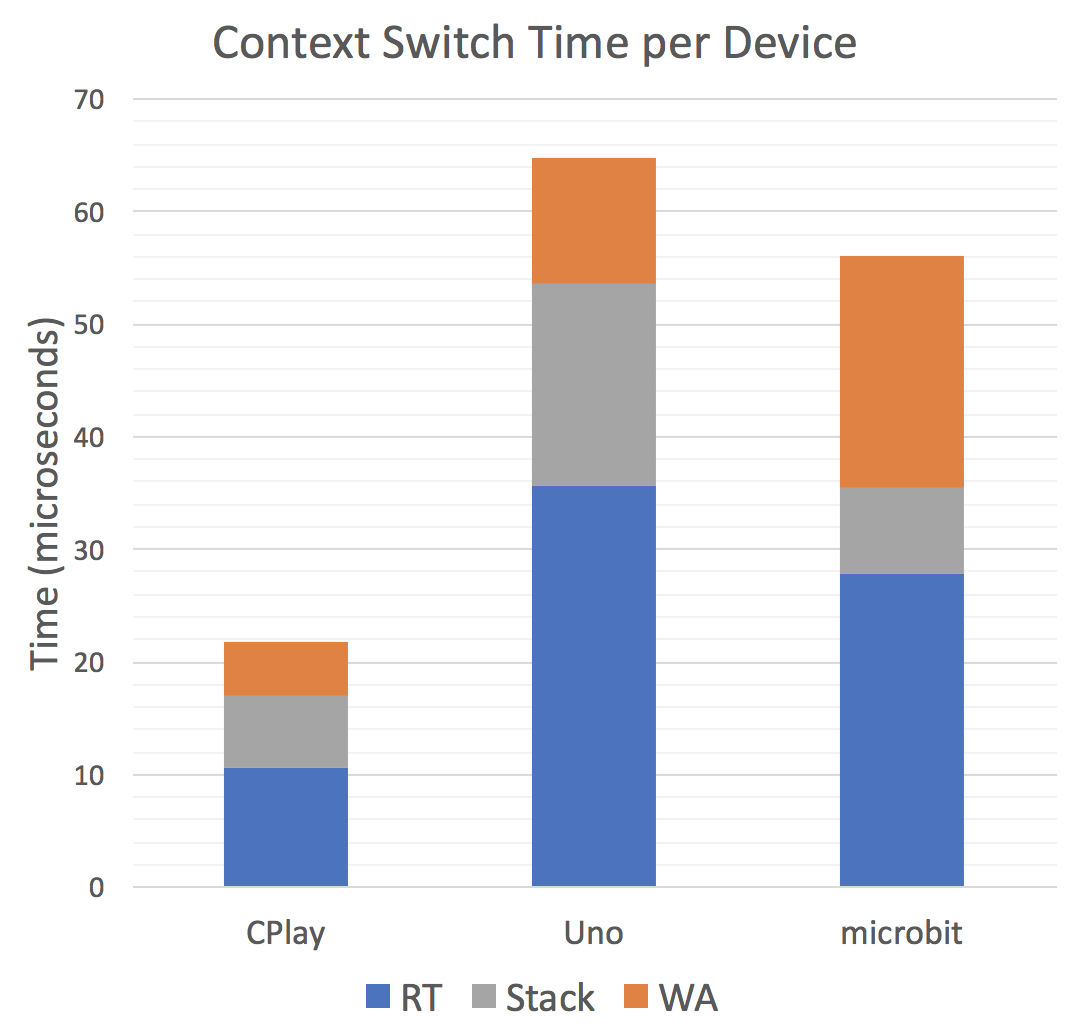
\includegraphics[width=.6\columnwidth]{images/context-switch.png}
\caption{\label{fig:context-switch}Base context switch profiles per device.}
\end{figure}

\begin{figure}[ht]
    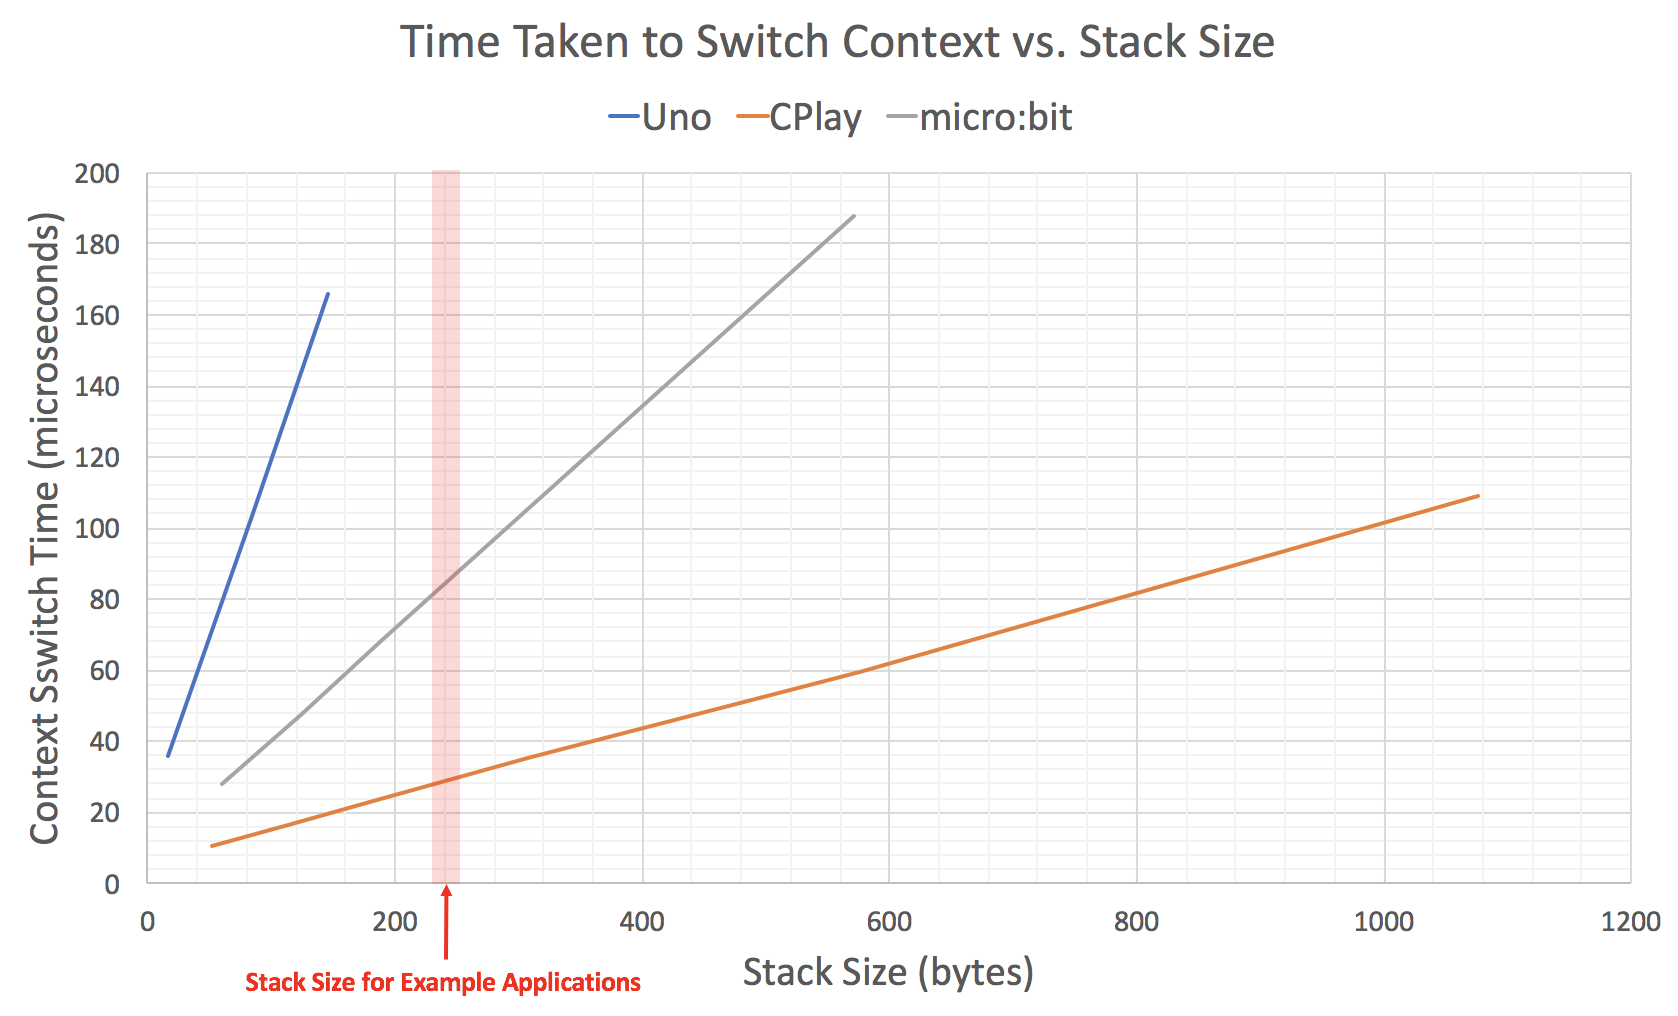
\includegraphics[width=.6\columnwidth]{images/context-vs-stack.png}
\caption{\label{fig:context-vs-stack}[UPDATE WITH RED BAR]Time taken to perform a context switch against stack size.}
\end{figure}

To evaluate the performance of the scheduler we conducted a test that created two fibers and continuously swapped context, in each fiber a GPIO was toggled enabling us to capture the duration using an oscilloscope. We performed this test in both \MC and \CO and the resulting profiles can be seen in Figure~\ref{fig:context-switch}. This figure breaks the context switch down into three phases: (1) \CO, the time it takes to perform a context switch in \CO; (2) Stack Swap, the time taken to page out the \MC stack; and (3) \MC, the overhead added by the \MC layer.

Figure~\ref{fig:context-vs-stack} profiles the time a context switch takes with an increasing stack size across all three devices in \CO. This test is similar to the previous test, however, we placed bytes (in powers of 2) on the stack of each fiber, starting from 64 and finishing at 1024. The difference in gradients, and ranges of values can be put down to device capability. For instance, the Uno has an 8-bit processor word size, which means more instructions are required to copy the stack, therefore as the stack size increases, so does context switch time.

\subsubsection{Asynchronous Operations}

% RENAME APC TO ASYNCHRONOUS PROC CALL and REORDER so that Event is below APC for ordering.
\begin{figure}[ht]
    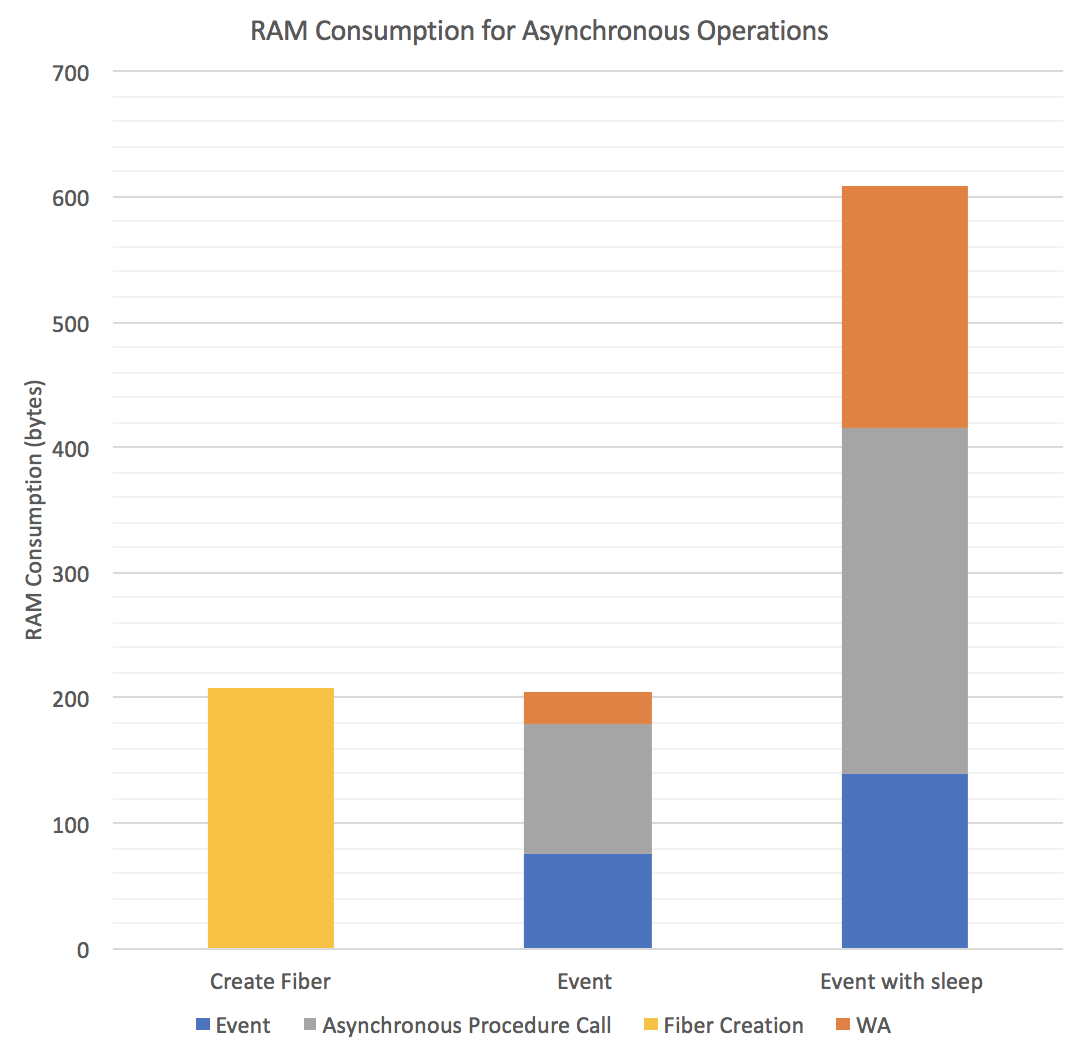
\includegraphics[width=.6\columnwidth]{images/ram-consumption.png}
\caption{\label{fig:ram-consumption}[NOT FINAL]RAM consumption of asynchronous operations in \CO.}
\end{figure}

\begin{figure}[ht]
    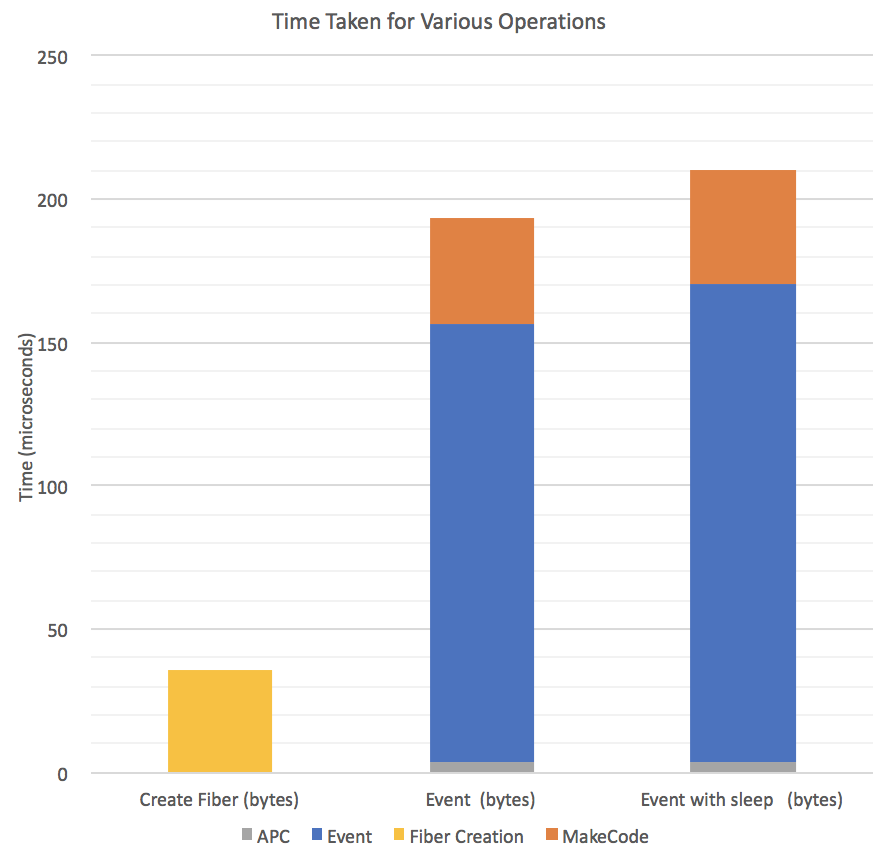
\includegraphics[width=.6\columnwidth]{images/time-taken.png}
\caption{\label{fig:time-taken}[NOT FINAL]Time taken to perform asynchronous operations in \CO.}
\end{figure}
To gauge the cost of different asynchronous operations in \CON, we tested three commonly used code paths using the CircuitPlayground: (1) creating a fiber; (2) handling a non-blocking event; and (3) handling a blocking event.

Figures~\ref{fig:ram-consumption}~and~\ref{fig:time-taken} show the RAM consumption and time taken to perform asynchronous operations in \CO, including the overhead of \MC where applicable.

In \CO, creating a fiber costs 208 bytes and 35.4 microseconds, a non-blocking event costs 180 bytes and 156.4 microseconds, and a blocking event costs 416 bytes and 170.4 microseconds. For a non-blocking event \MC adds 24 bytes and 36.8 microseconds, and for a blocking event it adds 192 bytes and 39.6 microseconds.

This exposes an optimisation made at the \CO layer, which is to only create a fiber to handle an event if a user performs a blocking operation in an event handler, as creating a fiber is a costly operation.

Handling an event consumes a lot of time, the reason for this is that once an event has been fired its' corresponding listener is looked up in a singley linked list, and then invoked.

\subsection{Memory Footprint}

\subsubsection{Flash Consumption}

\begin{figure}[ht]
    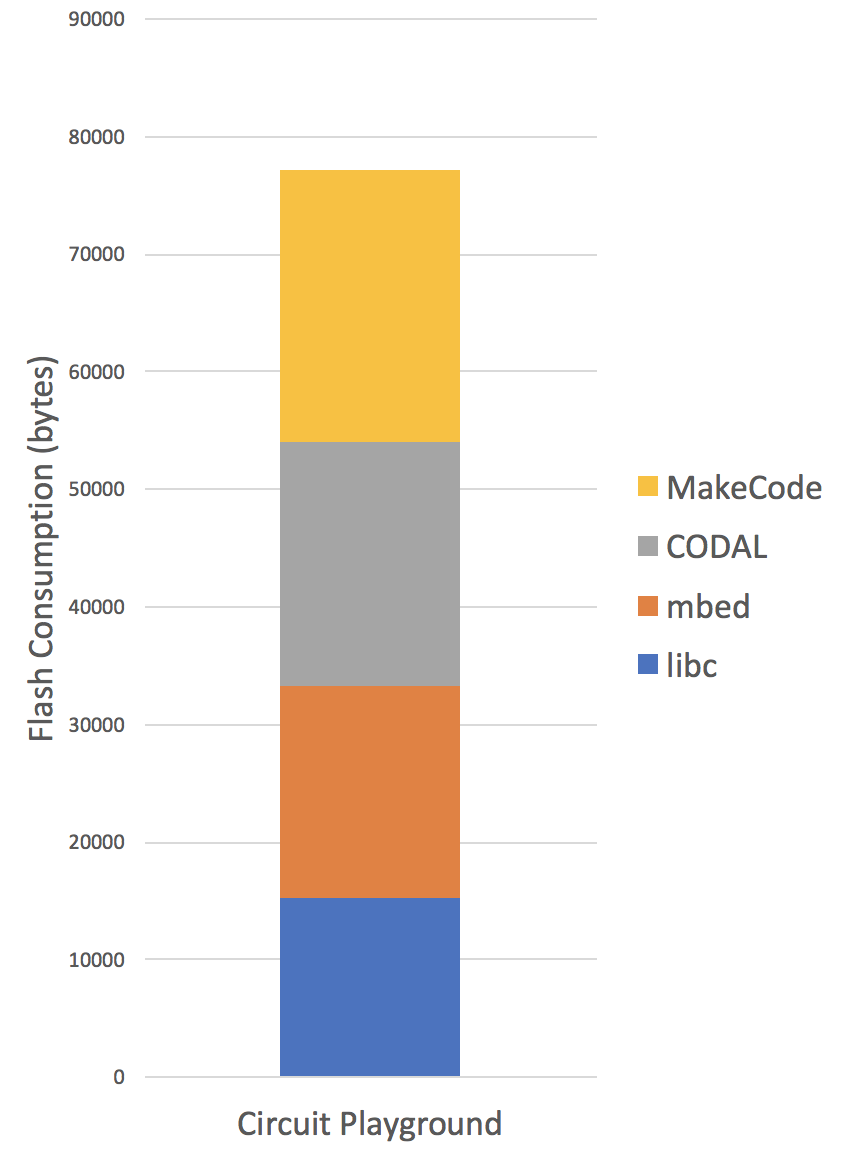
\includegraphics[width=.75\columnwidth]{./images/flash-consumption-per-device.png}
\caption{\label{fig:flash-consumption}The total flash consumption of code required to support \MC.}
\end{figure}

Figure~\ref{fig:flash-consumption} shows the flash consumption of each software library used in the final \MC binary. To obtain these numbers, we profiled the final map file produced after compilation. The stacked bars align with the composition of the software layer: \MC builds on \CO which builds on mbed and the C++ standard library.

From the bottom up, the profile of the standard library changes dramatically for each device: The uno has a very lightweight standard library; the microbit will uses 64-bit integer operations which will require extra standard library functions; and the CircuitPlayground requires virtualised floating point operations pulling in more standard library functions.

mbed is not used for the uno as it does not have an ARM processor. The micro:bit uses more of mbed than the CircuitPlayground, as over time we have begun to phase out mbed in favour of native implementations.

The size of \CO and \MC scales linearly with the amount of functionality a device has. For instance the uno has few onboard components when compared to the CircuitPlayground and micro:bit.

The configurability of \CO enables us to support multiple devices with different feature sets, whilst maintaining the same API at the \MC layer.

\subsubsection{RAM Consumption}
% Add globals maps and profile of listener and fiber.

% The CPX runtime is the largest, as the CPX device has lots of on-board
% components, and this runtime shares much of its code with other SAMD21 \MC targets.
% The compiled C++ runtime is 114k in total, with \CO accounting for 29k, with an
% additional 15k from libmbed. The \MCN-common-packages adds 20k, and also in
% an additional 49k of math support libraries (floating point operations,
% including trigonometry and number printing/parsing).
% As the SAMD21 has 256k of flash, we did not worry about optimizing this runtime for space.

% On the Uno, which has 32k of flash, the much \MC runtime is 8k and \CO is 14k (since
% the Uno only requires basic GPIO, i2c and serial drivers), leaving 10k for user code.

% The TypeScript part of the runtime is 1060 statements on the CPX and 216 on the Uno.
% In our microbenchmarks, 99\% of that runtime is tree-shaken away.

\subsection{\MC Native vs. \MC VM}

\subsection{Compiling Static TypeScript}
% data generated using 'node map-file-stats.js CIRCUIT_PLAYGROUND.map'
% maybe put it in a table?

% TOTAL 114.22
% pxtapp 20.46
% lib/gcc/arm-none-eabi/6.3.1/thumb/v6-m/crtbegin.o 0.09
% codal 29.72
% libmbed-classic.a 14.78
% lib/thumb/v6-m\libstdc++_nano.a 0.08
% lib/gcc/arm-none-eabi/6.3.1/thumb/v6-m\libgcc.a 12.76
% lib/thumb/v6-m\libm.a 24.28
% lib/thumb/v6-m\libc_nano.a 11.91
% lib/thumb/v6-m\libnosys.a 0.03

When compiling the Static TypeScript benchmarks and runtime with code shaking we obtain
a generated code density of 37.5 bytes per statement on CPX, 60.8 on AVR native, and 12.3 on AVR VM.
This excludes string literals (which don't change the picture significantly), but includes class
vtables and number literals if any. Note that ARM and AVR native instructions are 2 bytes each,
while AVR VM instructions are between 0.5 and 3 bytes.

When compiling, the entire TypeScript program, including the runtime, is
passed to the TypeScript (TS) language service for parsing. Then, only the remaining
part of the program (after code shaking) is compiled to native code.
On a modern laptop, using Node.js, TS parsing and analysis takes about 0.1ms per statement,
while \MC compilation to native code takes about 1ms per statement.
While the TS compiler has been optimized for speed,
\MCN's native compilation process hasn't been.
For example, for CPX the TS pass is dominated by compile the device runtime
and takes about 100ms, whereas the \MC pass typically only includes a small user program
and a small bit of the runtime, resulting in less than 100ms.
Thus, typical compilation times are in the range of 200ms for user programs
of ABC-XYZ lines.

The AVR VM was specifically designed for high code density, since the C++ runtime
leaves less than 10k for TS runtime and user code on the Uno.
The interpreter is implemented in assembly and always included with the program and is around 0.5k.
There are about 30 opcodes, some of which can take 1 or 2 byte arguments.
There are also a few combined opcodes, representing a sequence of one argument-less opcode,
and one with an argument, which improves code density by about 25\%.
Opcodes are direct offsets into the code of the interpreter, speeding up execution.
They operate on a stack (mainly for function calls) and a special scratch register.
There is essentially no stack space overhead compared to native AVR compilation.
The speed overhead is around 4x-5x (with respect to native) for computational tasks.


%\subsection{Implementation}
% •	\CO (SAMD21 and AVR): base runtime (C++ only)
% •	pxt
% •	pxt-common-packages: C++ and Static TypeScript
% •	pxt-adafruit
% •	pxt-arduino-uno
% •	pxt-monaco, pxt-blockly

%mmoskal [10:10 AM]
%`pxt checkdocs --snippets --re perf --stats`
% [10:11]
% I compile empty sample first twice, to reduce JIT costs
% [10:12]
% also, the first "compile prep" is slightly more costly, since it parses a hex file
